\chapter{Proofing}

\section{Basic Terminologies}

An \href{https://en.wikipedia.org/wiki/Axiom}{axiom}, postulate, or assumption (\textbf{tiên đề}, định đề) is a statement which we assume to be true without a proff. Sự thật hiển nhiên, luật chơi. Chúng ta không thể chứng minh tiên đề nên chấp nhận chúng.

A \href{https://en.wikipedia.org/wiki/Theorem}{Theorem} (định lý): an important result that has been proven. Pythagorean Theorem. The main goal of us is to prove theorems using mathematical proofs.

Definition: định nghĩa.

\textbf{Proposition} (mệnh đề): a statement that is either true of false. Chúng tuy không quá quan trọng (để được xếp vào nhóm định lý) nhưng vẫn thú vị.

A \textbf{Conjecture} (Sự giả định, giả sử): a statement that someone guesses to be true, although they are \textbf{not yet} able to prove or disprove it.

\textbf{Corollary} (hệ quả): a theorem that follows on from another theorem.

\textbf{Lemma} (bổ đề): a textit{small} result that has been proved. It is used to prove a theorem.

Proff by Induction : chứng minh bằng Phép quy nạp

contradiction: phản chứng

Deduce: suy ra

Proof: chứng minh

\section{Logical Rules}

Chấp nhận bằng niềm tin.

\noindent \textbf{Modus Ponens}: If p is true and p implies q, then q is true.

Logical notation: \(p,p \rightarrow q \therefore q\)

Example: p = ``It is raining'', q = ``The ground is wet''.

\textbf{Given}: ``It is raining'' and \q{It is raining implies the ground is wet}

\textbf{Conclusion}: \q{The groud is wet}

\vspace{4 mm}

\textbf{Modus Tollens}: If not q is true and p implies q, then not p is true.

Logical notation: \(\neg q, p \rightarrow q \therefore \neg p\)

Example: p = \q{It is raining}, q = \q{The ground is wet}.

\textbf{Given}: \q{The ground is not wet} and \q{It is raining implies the ground is wet}

\textbf{Conclusion}: \q{It is not raining}.

\vspace{10 mm}

\textbf{Hypothetical Syllogism}: If p implies q and q implies r, then p implies r.

Logical notation: \((p \rightarrow q), (q \rightarrow r) \therefore (p \rightarrow r)\)

\vspace{4 mm}

\textbf{Disjunctive Syllogism}: If not p is true and p or q is true, then q is true.

Logical notation: \(\neg p, (p \vee q) \therefore q\)

%===============================
\vspace{10 mm}

\textbf{Addition}: If p is true, then p or q is true.

Logical notation: \(p \therefore (p \vee q)\)

\vspace{4 mm}

\textbf{Simplification}: If p and q are true, then p is true.

Logical notation: \((p \wedge q) \therefore p\)

\vspace{4 mm}

\textbf{Conjunction}: If p is true and q is true, then p and q are true.

Logical notation: \(p,q \therefore (p \wedge q)\)

\section{Mathematical Sets}

A \href{https://en.wikipedia.org/wiki/Rational_number}{rational number} (số hữu tỉ) viết dưới dạng p/q trong đó p và q là số nguyên và q khác không; p is numerator (tử số) và q là denominator (mẫu số).

A \href{https://en.wikipedia.org/wiki/Real_number}{Real number} (số thực) bao gồm tất cả các số hữu tỉ, như số nguyên (5) và phân số \(\frac{2}{3}\), và tất cả các số vô tỉ, như \(\sqrt{2}, \pi\), v.v.

These are the common sets:

\begin{itemize}
  \item $\mathbb{N}$ --- The Natural Numbers (Counting Numbers): $\{1,2,3,...\}$
  \item $\mathbb{W}$ --- The Whole Numbers: $\{0,1,2,3,...\}$ non-negative integer.
  \item $\mathbb{Z}$ --- The Integers (số nguyên): $\{...,-3,-2,-1,0,1,2,3,...\}$
  \item $\mathbb{Q}$ --- The Rational Numbers: $\left\{ \frac{p}{q} \mid p,q \in \mathbb{Z}, q \neq 0 \right\}$
  \item $\mathbb{I}$ (commonly written as $\mathbb{R} \setminus \mathbb{Q}$) --- The Irrational Numbers: $\{x \mid x \not\in \mathbb{Q}, x \in \mathbb{R}\}$
  \item $\mathbb{R}$ --- The Real Numbers: $\{x \mid x \text{ can be written as a decimal}\} = \{x \mid x \in \mathbb{Q} \text{ OR } x \in \mathbb{I}\}$
  \item $\mathbb{C}$ --- The Complex (Imaginary) Numbers: $\{a+bi \mid a,b \in \mathbb{R} , i=\sqrt{-1}\}$
\end{itemize}

Some other common sets are:

\begin{itemize}
  \item $\mathbb{U}$ --- The Universal Set: \{All objects currently under discussion\}
  \item $\emptyset$ --- The Empty Set: \(\{\}\)
\end{itemize}

The \textbf{Cardinality} of a set is the number of distinct elements in the set. If the cardinality of a set is a whole number, we call it a \textbf{finite set}. Otherwise, we call it an \textbf{infinite set}.

\[|A| \text{ is the cardinality of set A}\]

Sets don't care about repetition or order.

\[ |\{1,2,2,3,3,3,4,4,4,4\}|=|\{4,3,2,1\}|=4 \]

\vspace{5 mm}

Set A and set B are \textbf{equal} (A=B) if

\begin{enumerate}
  \item Every element of A is an element of B
  \item Every element of B is an element of A
\end{enumerate}

(Both set contain exactly the same elements)

\[A \subseteq B\quad B \subseteq A\]

\vspace{7 mm}

A is a \textbf{Subset} of B, $A \subseteq B$, if every element of A is also an element of B.

\[
  \begin{aligned}
    &(a\in A \Longrightarrow a\in B)\\
    &\mathbb{N} \subseteq \mathbb{W} \qquad \mathbb{W} \not\subset \mathbb{N}
  \end{aligned}
\]

The \textbf{Power Set of A}, P(A), is the set of all possible subsets of A.

\vspace{10 mm}

The \textbf{Complement}, \(A^\complement \text{ or } A^\prime\), of a set A is the set of all elements in the universal set that are NOT elements of A.

\[
  \begin{aligned}
    &A^\complement = \{x \mid x \in \mathbb{U} \quad \text{and} \quad x \not\in A \}\\
    &A^\complement = \mathbb{U} \setminus A \text{ (This is the Set Difference or set minus notation)}
  \end{aligned}
\]

\vspace{8 mm}

The \textbf{Union} (hợp, hội) of two sets, $A \cup B$ is the set containing all the elements from either A or B.

\[A \cup B = \{ x \mid x \in A \text{ OR } x \in B \}\]

The \textbf{Intersection} (giao) of two sets, $A \cap B$, is the set of elements in both sets A and B.

\[a \cap B = \{ x \mid x\in A \text{ AND } x\in B \}\]

Two sets A and B are \textbf{Disjoint} if $A \cap B = \emptyset$

Theorem (\textbf{Transitive Property}): If $A \subseteq B \text{ and } B \subseteq C \text{ then } A \subseteq C$.

\section{Quantifiers}

\q{For all, for every} is the \textbf{Universal Quantifier} $\forall$

\q{There exists} is the \textbf{Existential Quantifier} $\exists$

Example:

\[
  \begin{aligned}
    &\forall\ y \in \mathbb{R},\ y^{2} \geq 0\\
    &\exists\ x \text{ such that } x+3=5
  \end{aligned}
\]

\textbf{Negations:}

\[
\begin{aligned}
  &\neg(A \text{ or } B) = \neg A \text{ and } \neg B\\
  &\neg(A \text{ and } B)= \neg A \text{ or } \neg B\\
  &\neg(\text{if } A,\ \text{then } B) = A \text{ and } \neg B\\
  &\neg (\forall\ x,y)= \exists\ x \text{ such that } \neg y\\
  &\neg (\exists x \text{ such that } y)= \forall x,\ \neg y\\
  &\neg (A \Longrightarrow B) = A \wedge \neg B\\
\end{aligned}
\]

For all M in the Real Numbers, there exists x in the Real Numbers such that the absolute value of $f(x)$ is greater than or equal to M.

\begin{equation}
  (\forall M \in \mathbb{R})\qquad (\exists x \in \mathbb{R})\qquad  \text{S.T.}\qquad  [|f(x)| \geq M]
  \label{statement01}
\end{equation}

Negations of statement \ref{statement01} above:

\begin{equation*}
  (\exists M \in \mathbb{R})\qquad \text{S.T.}\quad (\forall x \in \mathbb{R})\qquad  [|f(x)| < M]
\end{equation*}

\vspace{10 mm}

For all M in the Real Numbers there exists x in the Real Numbers such that for all y greater than than x we have $f(y)$ is greater than M.

\begin{equation}
  (\forall M \in \mathbb{R})\qquad (\exists x \in \mathbb{R})\qquad \text{S.T.}\qquad (\forall y > x)\quad [f(y) > M]  
  \label{statement02}
\end{equation}

Negations of statement \ref{statement02} above:

\begin{equation*}
  (\exists M \in \mathbb{R})\qquad \text{S.T.}\qquad (\forall x \in \mathbb{R})\quad (\exists y > x)\quad [f(y) \leq M]
\end{equation*}

For every epsilon greater than 0 there exists delta greater than 0 such that the absolute value of f(x) minus f(x initial) is less than epsilon when the absolute value of x minus x initial is less than delta.

\begin{equation}
  (\forall \varepsilon > 0)\quad (\exists \delta > 0)\quad \text{S.T.} \quad (\forall x \in \mathbb{R})\quad [|x-x_{0}| < \delta \Longrightarrow |f(x)-f(x_{0})| < \varepsilon]
  \label{statement2.3}
\end{equation}

Negations of statement \ref{statement2.3} above:

\begin{equation*}
  (\exists \varepsilon > 0)\quad \text{S.T.}\quad (\forall \delta >0)\quad (\exists x \in \mathbb{R})\quad \text{S.T.}\quad [|x-x_{0}| < \delta \wedge |f(x)-f(x_{0})| \geq \varepsilon]
\end{equation*}

\section{Direct Proofs}

Theorem: An even integer's square is also even.

Theorem: The square of an odd number is also odd.

Pythagorean Theorem: $a^{2}+b^{2}=c^{2}$ where a,b,c are sides of a right triangle. (c being the hypotenuse)

\section{Contrapositive}

\hl{Conditional Statement} (If-then statement): A statement with a hypothesis and a conclusion: If X, then Y. It can also be written as $X \rightarrow Y$.

Negation is written with a squiggly line (\textasciitilde) or the symbol ($\neg$).

Given a Conditional Statement, we can create four related statements:

\begin{itemize}
  \item Original Statement: If p, then q ($p \rightarrow q$)
  \item \hl{Converse}: If q, then p ($q \rightarrow p$). Interchange/switched the hypothesis and the conclusion. Nhớ \q{c} là \textbf{C}huyển đổi vị trí.
  \item \hl{Inverse}: If not p, then not q ($\neg p \rightarrow \neg q$). Take the negation of both the hypothesis and the conclusion)
  \item \hl{Contrapositive}: If not q, then not p ($\neg q \rightarrow \neg p$). Interchange the hypothesis and the conclusion of the inverse statement)
  \item Biconditionnal: $p \longleftrightarrow q$
\end{itemize}

If the statement is true, then the contrapositive is also logically true. If the converse is true, then the inverse is also logically true.

The most useful one in the real world is the converse.

\vspace{0.5cm}

To make the Contrapositive statement (Trái ngược, tương phản), the hypothesis and conclusion are switched \textbf{and} negated.

\[p \rightarrow q \equiv \neg q \rightarrow \neg p\]

\vspace{0.5cm}

\hl{Negation}: The opposite of an original statement.

Example 1: Original Statement The flowers are red. New Statement The flowers are not red

Example 2: Original Statement The number is not even. New Statement The number is even.

\vspace{.6cm}

\hl{Equivalent Statements}: Two statements that are either both true or both false.

Examples:

I) \colorbox{GreenYellow}{A statement and its contrapositive}.

Original Statement: If a polygon is a square, then it is a quadrilateral (tứ giác).

Contrapositve: If a polygon is not a quadrilateral, then it is not a Square. (also true)

\vspace{.4cm}

II) \colorbox{GreenYellow}{The converse and inverse}.

Converse: If a Polygon is a quadrilateral, then it is a square. (false)

Inverse: If a Polygon is not a square, then it is not a quadrilateral. (also false, counter-example hình thang trapezoid)

\section{If and Only If}

\q{If and Only If} or (iff) is the \textbf{Two Way Proof}. We must prove both the statement and its converse:

\[p \implies q \quad q \Longrightarrow p\]

\[p \iff q\]

\hl{Biconditional Statement}: A statement that is true, as well as its converse. It can be written with \q{if and only if}.

\begin{figure}[htb!]
  \centering
  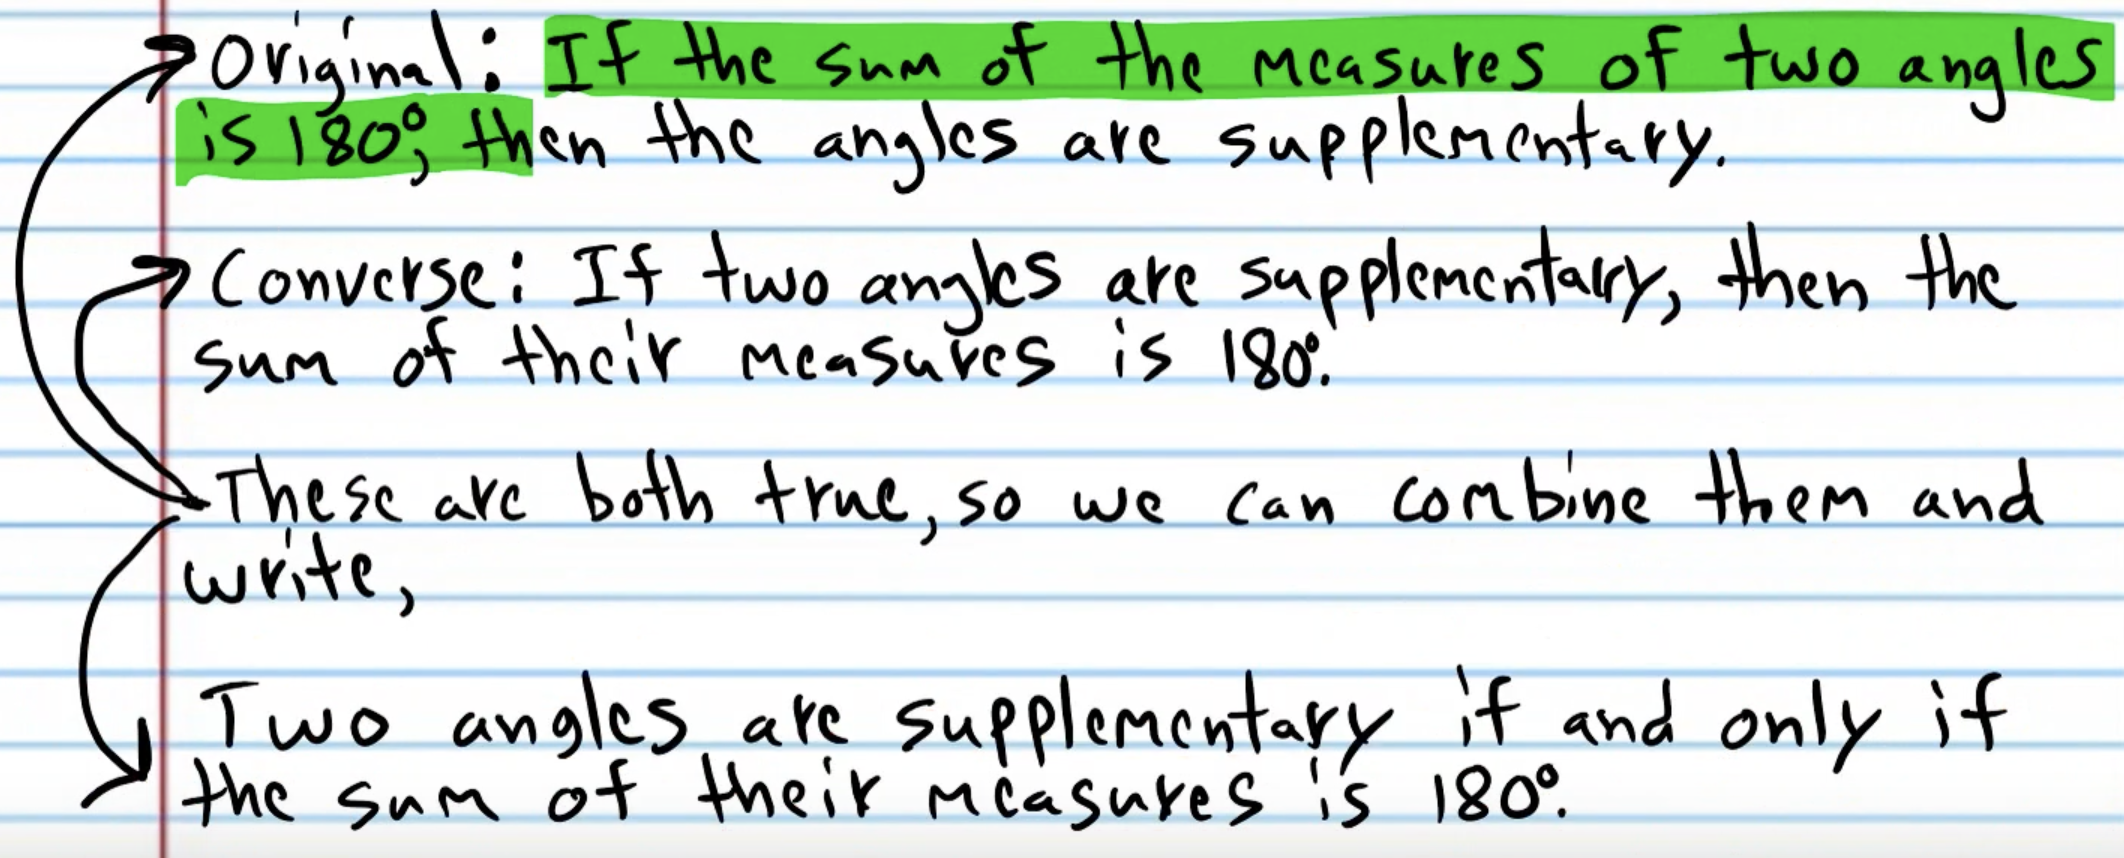
\includegraphics[width=0.8\textwidth]{biconditional-statement.png}
  \caption{Biconditional Statement}
\end{figure}

Definition statements are always biconditional-statement.

\section{Proof by Contradiction}

Assume the opposite of what we want to prove, then show a contradiction.

Prove $\sqrt{2}$ is irrational

\section{Theorems are always true}

Theorems can be \textbf{Disproven} with just one \textbf{Counter-Example}. And just provide some examples of Theorems are NOT suffice to be counted as a proofs.

A \textbf{Counter-example} to a mathematical statement is an example that satisfies the statement's condition(s) but does not lead to the statement's conclusion.

\section{Proof by Cases (Exhaustion)}

Chia ra cases rồi chứng minh từng cases.

Ví dụ cách chia case 01

\begin{itemize}
  \item Case 1: n is even
  \item Case 2: n is odd
\end{itemize}

Ví dụ cách chia case 02

\begin{itemize}
  \item Case 1: $x>=0$, $y>=0$
  \item Case 2: $x<0$, $y<0$
  \item Case 3: $x>=0$, $y<0$. Riêng case này có 2 sub-cases
\end{itemize}

\section{Mathematical Induction}

Let $P(n)$ be a statement for each $n \in \mathbb{N}$. If

\begin{enumerate}
  \item P(1) is true. (Base Case)
  \item P(k) is true implies $P(k+1)$ is true. (Induction Hypothesis)
\end{enumerate}

Then $P(n)$ is true for all $n \in \mathbb{N}$.

\vspace{.3cm}

An allegory regarding the domino effect is: (1) Knock down the first domino; (2) check that if a domino is knocked over, the next domino is also knocked over.

\vspace{0.5cm}

\hl{Inductive reasoning}: Drawing a conclusion based on a pattern taken from limited information.

\hl{Conjecture}: A conclusion based on \textbf{inductive} reasoning. It is not proofed. A conjecture can be wrong.

\vspace{.3cm}

\hl{Example I}: My cat has hair. Your cat has hair. The next door neighbor's cat has hair. Therefore, all cats have hair.

\hl{Example II}: It rained yesterday. It rained today. Therefore, it will rain every day of the year.

\hl{Example III}: Old Faithful, a geyser at Yellow-Stone National Park, is known to erupt many times per day since its discovery in 1870. Because this has always been true, it will continue to be true.

\vspace{0.3cm}

\hl{Counter-example}: An example that disproves a conjecture.

\section{Strong Iduction}

\textbf{Strong induction}, also known as complete induction, is a proof technique in mathematics used to prove that a statement is true for all natural numbers. It differs from regular induction in the inductive step, where instead of assuming only the statement holds for \(k\), it assumes the statement holds for all values up to and including $k$ and then prove that it is also true for $k+1$. If:

\begin{enumerate}
  \item $P(r)$ is true
  \item $P(j)$ true => $P(k+1),\ r\leq j \leq k$
\end{enumerate}

Then $P(n)$ is true $\forall n\in \mathbb{N}, (r \leq n)$

\section{Deductive Reasoning}

\hl{Deductive Reasoning}: An argument based on definitions, postulates, theorems, and logic.

\vspace{.4cm}

\hl{The Law of Detachment} (Modus Ponens): If $X \rightarrow Y$ is true, and X is true, then Y must be true.

Example:

If I hurt my arm, then I will not be able to pitch in the game tomorrow.

If it is true that an injury to my arm will prevent me from pitching in the game, and if it is also true that my arm has been, injured, then the conclusion, I will not be able to pitch in the game tomorrow, must also be true.

\vspace{.5cm}

\hl{The Law of Syllogism} (tam đoạn luận): If $X \rightarrow Y$ is true, and $Y \rightarrow Z$ is true, then $X \rightarrow Z$ must be true.

Example: If I lost my car keys, then I will be late to the party. If I am late to the party, then the host will be angry.

Therefore, if I lose my car keys, then the host of the party will be angry.

\section{Introduction to Functions}

A function f: A -> B is a mapping from a set of A (domain) to a set of B (co-domain), such that $\forall x\in A, \exists !y \in B$, where $f(x)=y$.

Domain (D): set of all possible inputs.

Codomain (B): set of all possible outputs.

Range (R): set of all actual outputs. It's a sub-set of the codomain.

Some special types of functions:

\begin{itemize}
  \item \textbf{Injective}: $\forall x_{1}, x_{2}\in D, f(x_{1})=f(x_{2}) \Rightarrow x_{1}=x_{2}$. Distinct inputs have distinct outputs.
  \item \textbf{Surjective}: $\forall y \in R, \exists x \in D : f(x)=y$. Every output has at least one input.
  \item \textbf{Bijective}: Injective and Surjective. One-to-one correspondence.
\end{itemize}

\section{Existence Proof}

Chỉ cần tìm ra một element thỏa điều kiện là xong.

Ví dụ:

Theorem: There exists an integer n with the property $|n^{2}-5| \leq 1$

\section{Uniqueness Proofs}

\textbf{Definition}: Prove only one element satisfies the conditions of a statement. Có thể chia làm 2 phần:

\begin{itemize}
  \item \textbf{Proving Existence}: Show at least one element satisfies the conditions
  \item \textbf{Proving Uniqueness}: Show no other element satisfies the conditions.
\end{itemize}

Example:

Prove that 2 is the unique positive number that is both prime and even.

\section{False Proofs}

A \textbf{False Proof} is one that, on the surface, might look correct, but ultimately, has an error in it. Once you spot that error, we conclude the proof is invalid.

\section{Fundamental Theorem of Arithmetic}

A Prime Number is a whole number above 1 that \textbf{cannot} be made by multiplying other whole numbers. Prime Numbers in math are like the elements in Chemistry. That is, they are the most basic building blocks from which all numbers are created. By multiplying prime numbers we can create any other whole number.

A prime number cannot be exactly divided by any other number (except 1 and itself).

\vspace{8 mm}

The \textbf{Basic Idea} is that any integer above 1 is either a Prime Number, or can be made by \textbf{multiplying Prime Numbers} together (a \textbf{unique} product of prime numbers, ignoring the order).

\textbf{Prime Factorization:} The prime numbers when multiplied equal the number

\vspace{10 mm}

\textbf{Greatest Common Factor} (ước số chung lớn nhất): the largest positive integer that divides each of the integers.

To find GCF: list the prime factor of each number, multiply those factors that are in common.

GCF of 24 and 36:

\[
  \begin{aligned}
    24 &= 2^{3} \cdot 3\\
    36 &= 3^{2} \cdot 2^{2}\\
    \rightarrow \text{GCF} &= 2^{2} \cdot 3 = 12
  \end{aligned}\]
\[\]

\textbf{Least Common Multiple} (bội chung nhỏ nhất): the smallest positive integer that is divisible by both a and b. số nguyên dương nhỏ nhất chia hết cho cả a và b.

\section{Divisibility}

In mathematics, \href{https://en.wikipedia.org/wiki/Parity_%28mathematics%29}{parity} (tính chẳn lẻ) is the property of an \textbf{integer} of whether it is even or odd.

The above definition of parity applies ONLY to integer numbers, hence it cannot be applied to numbers with decimals or fractions like 1/2 or 4.6978. See the section "Higher mathematics" below for some extensions of the notion of parity to a larger class of "numbers" or in other more general settings. 

An even number is an integer of the form

\[x=2k,\ (k \in \mathbb{Z})\]

\vspace{10 mm}

The phrase \q{2 divides x} means that \textbf{x is divisible by 2} — in other words, when you divide x by 2, the result is a whole number and the remainder is 0.

\[2 \mid x \text{ means } \exists k \in \mathbb{Z} \text{ such that } x = 2k\]

\q{Divisible By} means when you divide one number by another the result is a \textbf{whole number} and the remainder is 0.

\begin{itemize}
  \item 14 \textbf{is} divisible by 7, because $14 \div 7 = 2$ \textbf{exactly}
  \item 15 is \textbf{not} dibisible by 7, because $15 \div 7 = 2\frac{1}{7}$ (the result is not a whole number)
  \item 0 \textbf{is} divisible by 7, because $0 \div 7 = 0$ exactly (0 is  whole number)
\end{itemize}

\q{Divisible by} and \q{can be exactly divided by} mean the same thing.

\subsection{The Divisibility Rules}

Zero is divisible by \textbf{any number} (except itself), so get a \q{yes} to all these tests.

\textbf{1} Any integer (not a fraction) is divisible by 1

\textbf{2} The last digit is even (0,2,4,6,8)

\begin{itemize}
  \item 128 => Yes
  \item 129 => No
\end{itemize}

\textbf{3} The sum of the digits is divisible by 3

\begin{itemize}
  \item 381 ($3+8+1=12$, and $12 \div 3 = 4$) \textbf{Yes}
  \item 217 ($2+1+7=10$, and $10 \div 3 = 3\frac{1}{3}$) \textbf{No}
\end{itemize}

\vspace{10 mm}

\textbf{4} The last two digits are divisible by 4

\begin{itemize}
  \item 1312 is ($12 \div 4 = 3$) \textbf{Yes}
  \item 7019 \textbf{No}
\end{itemize}

We can also substract 20 as many times as we want before checking:

\begin{itemize}
  \item 68: subtract 3 lots of 20 and we get 8 \textbf{Yes}
  \item 102: subtract 5 lots of 20 and we get 2 \textbf{No}
\end{itemize}

Another method is to \textbf{halve the number twice} and see if the result is still a whole number:

\begin{itemize}
  \item 124/2 = 62, 62/2 = 31, and 31 is a whole number. \textbf{Yes}
  \item 30/2 = 15, 15/2 = 7.5 which is not a whole number. \textbf{No}
\end{itemize}

\vspace{10 mm}

\textbf{5} The last digit is 0 or 5

\begin{itemize}
  \item 175 \textbf{Yes}
  \item 809 \textbf{No}
\end{itemize}

\textbf{6} Is even and is divisible by 3 (it passes both the 2 rule and 3 rule above)

\begin{itemize}
  \item 114 (it is even, and $1+1+4=6$ and $6 \div 3 =2$) \textbf{Yes}
  \item 308 (it is even, but $3+0+8=11$ and $11 \div 3 = 3\frac{2}{3}$ \textbf{No}
\end{itemize}

\textbf{7} Double the last digit and subtract it from a number made by the other digits. The result must be divisible by 7. (We can apply this rule to that answer again)

\begin{itemize}
  \item 672 (Double 2 is 4, $67-4=63$, and $63 \div 7 = 9$) \textbf{Yes}
  \item 105 (Double 5 is 10, $10-10=0$, and 0 is divisible by 7) \textbf{Yes}
  \item 905 (Double 5 is 10, $90-10=80$, and $80 \div 7 =11\frac{3}{7}$) \textbf{No}
\end{itemize}

\vspace{7 mm}

\textbf{8} The last three digits are dibisible by 8

\begin{itemize}
  \item 109816 ($816 \div 8=102$) \textbf{Yes}
  \item 216302 ($302\div 8=37\frac{3}{4}$) \textbf{No}
\end{itemize}

A quick check is to halve three times and the result is still a whole number:

\begin{itemize}
  \item 816/2 = 408, 408/2 = 204, 204/2 = 102 \textbf{Yes}
  \item 302/2 = 151, 151/2 = 75.5 \textbf{No}
\end{itemize}

\vspace{7 mm}

\textbf{9} The sum of the digits is divisible by 9. This rule can be repeated when needed.

\begin{itemize}
  \item 1629 ($1+6+2+9=18$, and again $1+8=9$) \textbf{Yes}
  \item 2013 ($2+0+1+3=6$) \textbf{No}
\end{itemize}

\textbf{10} The number ends in 0

\begin{itemize}
  \item 220 \textbf{Yes}
  \item 221 \textbf{No}
\end{itemize}

\textbf{11} Add and subtract digits in an alternating pattern (add digit, subtract next digit, add next digit, etc). Then check if that answer is divisible by 11.

\begin{itemize}
  \item 1364 ($+1-3+6-4=0$) \textbf{Yes}
  \item 913 ($+9-1+3=11$) \textbf{Yes}
  \item 3729 ($+3-7+2-9=-11$) \textbf{Yes}
  \item 987 ($+9-8+7=8$) \textbf{No}
\end{itemize}

\vspace{7 mm}

\textbf{12} The number is divisible by both 3 \textbf{and} 4 (it passes both the 3 rule and 4 rule above)

\begin{itemize}
  \item 648
  \item (By 3? $6+4+8=18$ and $18\div 3=6$ Yes)
  \item (By 4? $48\div 4=12$ Yes)
  \item Both pass, so \textbf{Yes}
\end{itemize}

\begin{itemize}
  \item 524
  \item (By 3? $5+2+4=11$, $11\div 3=3\frac{2}{3}$ No)
  \item (Don't need to check by 4) \textbf{No}
\end{itemize}

\subsection{Factors can be useful}

Factors are the numbers you multiply to get another number. In $2 \times 3=6$, 2 and 3 are the two factors.

When a number is divisible by another number then it is \textbf{also} divisible by each of the factors of that number.

\begin{itemize}
  \item If a number is divisible by 6, it is also divisible by 2 and 3
  \item If a number is divisible by 12, it is also divisible by 2, 3, 4 and 6.
\end{itemize}

\subsection{Euclid's lemma}

In mathematics, a lemma is a proven proposition that serves as a stepping stone to proving a larger or more significant theorem.

\textbf{Euclid's lemma}—If a prime p divides the product $ab$ of two integers a and b, then p must divide at least one of those integers a or b (one or both).

If p is prime and p | $ab$, then p | a or p | b
